\chapter{Applications}
\label{chap:clients}

In Chapter \ref{chap:purpose} I discussed several potential
applications for Custos. In Chapter \ref{chap:platform} I discussed
the Custos architecture and server API. In this chapter, I'll look
more closely at several example applications that interface with the
Custos server and leverage Custos to enhance their functionality. As
with the implementations provided in Chapter \ref{chap:platform},
these applications are designed merely to serve as examples of how one
might leverage Custos. They are by no means intended to represent a
complete list of all possible Custos applications. Nor are they
designed as fully production ready systems. They are proofs of concept
that demonstrate how to use Custos and the features using Custos
brings.

\section{\texttt{EncFS}: A Custos-backed Encrypted File System}

As discussed, encrypted file systems are a core Custos use case. As
such, I have written a layered, encrypted pass-through file system:
\texttt{EncFS}. This file system leverages Custos for encrypted file
key storage, and leverage underlying file systems for encrypted file
storage. It enables use cases not normally available in other
encrypted file systems.

The file system is capable of supporting encrypted operation in a wide
range of scenarios. Since it is a pass-through file system, it can be
used atop Cloud storage systems like Dropbox~\cite{dropbox}, secure
storage of a users files in the cloud. Custos enables access to the
encrypted files from multiple devices or by multiple users, allowing a
user to use Dropbox as they normally would to sync files across
multiple devises or to share files with other, all while still
benefiting from client-side encryption.

The system can also be used atop a user's local file system, guarding
against data compromise in the event that the user's computer is lost
or stolen. In addition, the file system has proven useful for use on
servers, where Custos's flexible authentication systems can allow for
daemon-based non-interactive access. This has allowed me to encrypt
server files like logs or mailboxes that normally must not be
encrypted in order to support non-interactive access by system
processes.

\subsection{Architecture}

\begin{figure}[!tb]
  \vspace{5ex}
  \begin{center}
    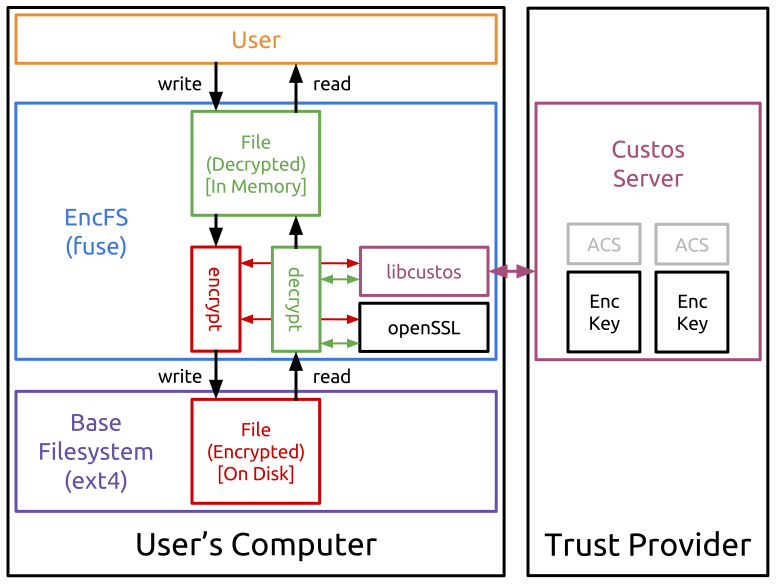
\includegraphics[width=.75\textwidth]
                    {./figs/pdf/App-FS-Fuse.pdf}
  \end{center}
  \caption{The \texttt{EncFS} File System Architecture}
  \label{fig:app-encfs}
\end{figure}

As Figure \ref{fig:app-encfs} shows, \texttt{EncFS} uses an
architecture similar to that described as the ``layered model'' in
Chapter \ref{chap:purpose}. It acts as a shim between file system
operations (read, write, create, etc) and the actual realization of
these operations on the underlying file system, providing transparent
encryption in the process. If the user attempts to read a file
directly from disk without first passing through the \texttt{EncFS}
layer, they will only received encrypted gibberish. But when the same
file is accessed through the \texttt{EncFS} layer, the user may
interact with the file as though it were not encrypted at all. As
such, the user's files are fully protected when the \texttt{EncFS}
layer is not running, and easily accessible when this layer is
running.

At this time \texttt{EncFS} only provides file encryption, not file
organization (directory structure) encryption. This is sufficient to
demonstrate how to use Custos to secure an encrypted file system,
while avoiding the complexity of also encrypting file system
organization. When a user wishes to start \texttt{EncFS}, they specify
a mount point and a base file system point. The base file system point
becomes the root of the \texttt{EncFS} backing file system. Any files
accessed via the \texttt{EncFS} mount point are actually
stored/accessed at the underlying base file system
point. \texttt{EncFS} simply provides a means for adding and removing
encryption between the actual storage of files on the underlying file
system and the corresponding access to files on the part of a user.

Because file systems do nor normally provide means for interactive
authentication, all necessary authentication parameters must be passed
to \texttt{EncFS} at the time it is mounted/started. If a user tries
to access a file for which the combination of provided and implicit
authentication attributes are not sufficient, they are simply denied
access to the file. \texttt{EncFS} itself does not provide the ability
to manipulate Custos Access Control Specifications. Instead, this
manipulation is handled by a separate, dedicated utility program (see
below). As long as the user has the necessary permissions, all
encrypted file access via \texttt{EncFS} is fully transparent,
allowing easy integration with other applications via the standard
Linux file interface~\cite{linux-vfs}.

\subsection{Implementation}

\texttt{EncFS} is implemented using the FUSE~\cite{fuse} user-space
file system framework. I chose a FUSE-based implementation over a
native Linux kernel-module implementation for \texttt{EncFS} in order
to allow easy usage of a variety of user-space libraries
(i.e. \texttt{libcustos}, OpenSSL, etc). The basics of using FUSE to
create a virtual overlay file system like \texttt{EncFS} are
described in my previous work: ~\cite{sayler-os-encfs}. FUSE provides
a series of callbacks that are triggered by various file system
operations. Each callback is then implemented by \texttt{EncFS} in C
in order to provided the desired encryption functionality.

All encryption in \texttt{EncFS} uses the AES symmetric encryption
cipher with 256-bit keys and the CBC encryption mode. Encryption
operations are handled by the OpenSSL~\cite{openssl} crypto
library\footnote{Following the old adage that one should never ``roll
  their own'' crypto. Leave it to the professionals! (Or at least to a
  widely used, well vetted, open-source code base.)}. Data written via
the \texttt{EncFS} mount point is encrypted before being committed to
an actual file on the underlying disk. Likewise, data read via the
\texttt{EncFS} mount point is decrypted before being passed back to
the user. This includes decrypting files when the user accesses
related meta-data like file size to ensure the user receives the size
of the unencrypted file content. Currently, \texttt{EncFS} encrypts
files in single CBC blocks, meaning the entire file must be read to
decrypt any portion of it. This can have an adverse effect on access
to random offsets within a file. I plan to upgrade the system to
support breaking files into blocks in order to speed random access and
streaming operations in the near future.

\texttt{EncFS} interacts with Custos via the \texttt{libcustos}
library (see Chapter \ref{chap:platform}). This allows \texttt{EncFS}
to offload the complexities of the Custos API to a dedicated code
base. \texttt{libcustos} provides the necessary functions to allow
\texttt{EncFS} to read, update, delete, and create Custos key:value
objects. When a user wishes to decrypt a file, \texttt{EncFS}
requested the associated encryption key from the Custos server using
the UUID stored with the file (either via extended attributes or in a
header block appended to the encrypted file contents, depending on
underlying file system support for extended attributes). If
\texttt{EncFS} posses the necessary authentication attributes (either
supplied by the user at mount time or derived contextually), Custos
returns the requested encryption key and \texttt{EncFS} proceeds to
decrypt the file. The opposite operation occurs when a file is created
or written, with \texttt{EncFS} rotating the encryption key and
uploading a new version to Custos for each write operation.

\section{``Banking'' Website}

As a second example application, I've designed the shell of a fake
``banking'' website (meant to represent any website that collects
personal data) that demonstrates how a user and website could use
Custos as a dedicated user data store (instead of the more typical
encryption key store discussed in the previous example). This example
presents the user with a basic ``Enter your info'' page familiar to
anyone who has ever signed up for a web site user account. Unlike a
normal ``Enter your info'' page, however, instead entering their info
directly, the user instead inputs a UUID pointing to the corresponding
info on a Custos server. If the website wishes to read this info, the
user must grant them read access to the associated object on the
Custos server. This allows the user to control and audit website
access to data. It also allows the user to avoid having to reenter or
update the same data on multiple websites. The user leverages Custos
as a single repository of all her data, granting websites access to
specific data objects as required.

\subsection{Architecture}

\begin{figure}[!tb]
  \vspace{5ex}
  \begin{center}
    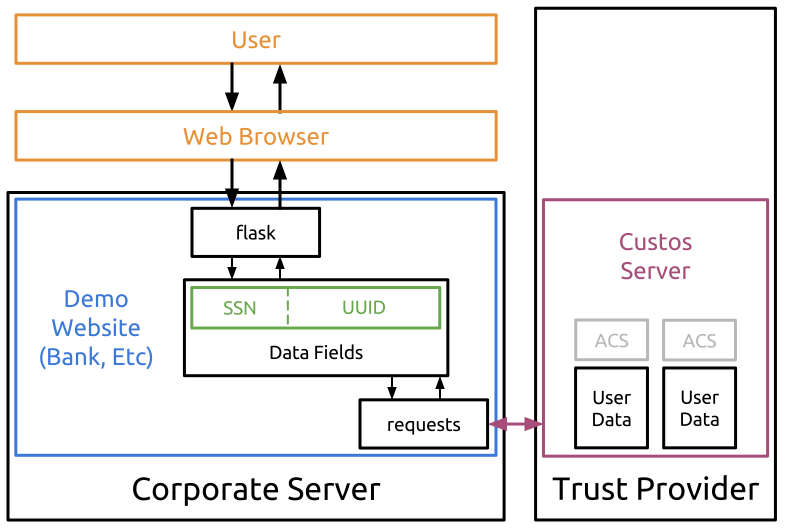
\includegraphics[width=.75\textwidth]
                    {./figs/pdf/App-SS.pdf}
  \end{center}
  \caption{The Demo ``Banking'' Website Architecture}
  \label{fig:app-bank}
\end{figure}

Figure \ref{fig:app-bank} shows the basic structure of the ``banking''
website demo app. The user is presented with an ``create new account''
page that prompts her for a variety of personal information (Name,
SSN, address, etc). The user provides a UUID in response to each of
these prompts instead of providing the data directly. The user is
assumed to have already created the corresponding data objects on a
Custos server (via the management interface discussed next).

When the user is done producing UUIDs, the website attempts to access
this data on the Custos server and display it to the user. If the user
has granted the website read access to the data (e.g. via a unique
access key displayed to the user when entering the UUIDs, IP address,
or various other attributes or combinations of attributes), the server
will return the data which the website can then store. As discussed in
Chapter \ref{chap:purpose}, this both saves the user the hassle of
manually entering data, and also saves the website the trouble of
locally storing data and keeping it safe and up to date. The user also
gains the benefit of the ability to revoke this data access latter and
to audit when and how the website is accessing the data.

\subsection{Implementation}

The website is implemented in Python 2.7 using the
Flask~\cite{python-flask} microframework (similar to the process
format used to implement the Custos server in Chapter
\ref{chap:platform}, but with actual UI elements instead of just a
RESTful API). The application communicates with the Custos server via
the Python requests~\cite{python-requests} module. Python's numerous
standard modules handle JSON processing, Base64 decoding, etc making
interfacing a Python application directly with the Custos server far
easier than implementing a Custos-backed C application. Thus, no
specialized library (i.e. \texttt{libcustos}) is necessary.

When the user loads the website, it displays a basic form to the user,
composed of the requested data fields and a unique website ID key,
randomly generated for each user and kept as a secret between the user
and the website. The user can (optionally) use this key as an
authentication attribute when limiting access to their data on the
Custos server to uniquely identify a specific website. When the user
submits the form, the web app attempts to query the Custos server for
the provided UUIDs, sending along the secret key it displayed to the
user as an authentication attribute. If the user has granted the site
read access to her data, either using this key, the server IP address,
some other attribute, or a combination of several attributes, the
Custos server returns the data which is then displayed to the user for
verification.

\section{Custos Management UI}

In order to make Custos data easy to manage while developing various
Custos apps that lack built-in management capabilities, I've designed
a basic management user interface that simplifies the process of
interacting with the Custos server. It provides a means to directly
managing the Access Control Specification associated with a given
Custos key:value object, as well as to directly read and write
objects.

\subsection{Architecture}

\begin{figure}[!tb]
  \vspace{5ex}
  \begin{center}
    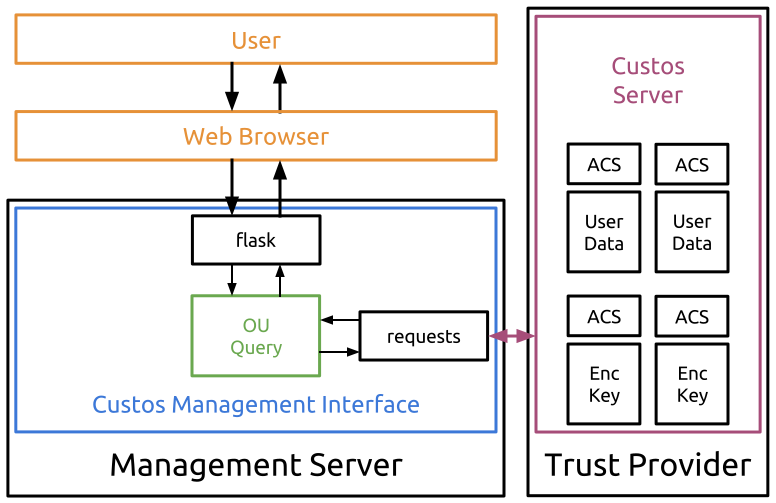
\includegraphics[width=.75\textwidth]
                    {./figs/pdf/App-Mgmt.pdf}
  \end{center}
  \caption{The ACS Management Architecture}
  \label{fig:app-mgmt}
\end{figure}

The management interface utilizes a web-based UI for managing Custos
access control specifications and key:value data (Figure
\ref{fig:app-mgmt}). The user accesses the UI by ``logging in''
through the prevision of one or more authentication attributes. The UI
stores these attributes in the user's resulting session state, and
leverages them to provide the user access to various Custos
permissions. The user must have the ability to gain the appropriate
permissions in order to make effective use of the management UI.

Once ``logged in'', the user can input a UUID identifying a Custos
key:value object, or request to create a new object. They may then
choose to view the object and/or the current ACS associated with the
object. At this point, they can make any changes they desire to either
the object or the ACS before re-uploading the object or ACS to Custos
(assuming they ``logged on'' with the appropriate permissions,
otherwise their request will be denied). It is possible to list
multiple objects in order to perform batch changes.

Custos's flexible authentication system also allows the administrator
to setup Custos to allow management access to any request from a
specific IP, making it simple to designate a management machine that
can fully control Custos access without requiring more complex
attributes. This method has been used effectively to provide
\texttt{local-host} access to a Custos server to expedite management
of server data while developing against it. It provides a means to
manage the ACSs associated with encrypted files from the
\texttt{EncFS} application, as well as the means to store user data
and manipulate allowed viewers in the ``Banking'' Website application.

\subsection{Implementation}

Like the Custos server and the ``Banking'' website, the management UI
is implemented in Python using Flask. It initially prompts the user to
``login'' by providing one or more authentication attributes in
JSON. These are then associated with the user's session state within
the Flask framework.

When a user request to create or view an ACS or key:value object, the
back-end builds the necessary Custos message and issues the request,
appending the users supplied authentication attributes to the
request. If the user has the necessary permissions to view the request
item, the item is returned. The user can manipulate the existing item
directly, and if she desires, send it back to Custos, replacing the
original item, again, assuming the necessary permission. This system,
while not the most polished, provides the user with the ability to
fully manipulate any item in the Custos stored object.

The management interface could also be coded as a command line utility
with fairly minimal changes. The interface would be similar, just via
command line interaction instead of a web UI. Neither system is ideal
for large scale, production Custos management, but both are adequate
for basic Custos management while testing or using the system with
only a few users.

%%  LocalWords:  EncFS libcustos OpenSSL ACSs ACS
